\documentclass[a4paper, 12pt]{article}

\usepackage[utf8]{inputenc}
\usepackage[T1]{fontenc}
\usepackage{textcomp}
\usepackage{listings}
\usepackage{lmodern}
\usepackage{amsfonts}
\usepackage{titling}
\usepackage{lipsum}
\usepackage[left=1in, right=1in, bottom=1in, top=1in]{geometry}
\usepackage{amsthm}
\usepackage{tcolorbox}
\usepackage{hyperref}
\usepackage{xcolor}
\usepackage{graphicx}
\usepackage{makeidx}
\usepackage{tikz}
\usepackage{pgfplots}
\pgfplotsset{compat=1.18}
\usetikzlibrary{shapes.geometric, calc}
\usepackage{svg}
\usepackage{amsmath, amssymb}
\usepackage{cases}
\usepackage{tkz-berge}
\usepackage{url}
\usepackage{tgtermes}
\usepackage{sectsty}
\usepackage{subcaption}
\usepackage{setspace}
\usepackage{float}
\usepackage{appendix}
\usepackage{pdflscape}
\usepackage[
    style=apa,
    backend=biber
]{biblatex}

\addbibresource{references.bib}

\definecolor{tugblue}{HTML}{33588B}
\allsectionsfont{\color{tugblue}}
\newcommand{\coloredrule}[2][tugblue]{%
  \textcolor{#1}{\rule{\linewidth}{#2}}%
}

\usepackage{import}
\usepackage{xifthen}
\usepackage{pdfpages}
\usepackage{color}
\newcommand{\incfig}[2][1]{%
    \def\svgwidth{#1\columnwidth}
    \import{./figures/}{#2.pdf_tex}
}

\theoremstyle{plain}
\newtheorem{thm}{Theorem}[section]
\newtheorem{lem}[thm]{Lemma}
\newtheorem{prop}[thm]{Proposition}
\newtheorem*{cor}{Corollary}

\theoremstyle{definition}
\newtheorem{defn}{Definition}[section]
\newtheorem{conj}{Conjecture}[section]
\newtheorem{exmp}{Example}[section]
\newtheorem{axiom}{Axiom}
\theoremstyle{remark}
\newtheorem*{rem}{Remark}
\newtheorem*{note}{Note}

\definecolor{darkgreen}{rgb}{0.0, 0.5, 0.0}

\lstset{
  language=bash,
  morekeywords={sysbench, fio, sudo, swapoff},
  morekeywords=[2]{--cpu-max-prime, --threads, --time, --memory-block-size,
    --memory-total-size, --name, --ioengine, --rw, --bs, --size,
    --numjobs, --runtime, --group_reporting},
  keywordstyle=[2]\color{tugblue!70},
  basicstyle=\small\ttfamily,
  breaklines=true,
  frame=single,
  rulecolor=\color{tugblue},
  backgroundcolor=\color{tugblue!5},
  numbers=left,
  numberstyle=\tiny\color{tugblue},
  xleftmargin=2pt,
  captionpos=b,
  showstringspaces=false,
  commentstyle=\color{darkgreen},
  keywordstyle=\color{tugblue}\bfseries,
  stringstyle=\color{red},
  columns=flexible,
}
\begin{document}
	\begin{titlepage}
        \vspace*{0.8cm}
        \begin{center}
           \coloredrule{2pt}\par
            \vskip 0.6cm
            \textbf{\Huge Virtualisation and Cloud Technologies}\par
            \vskip 0.3cm
            \coloredrule{2pt}\par

            \vskip 3cm
    
            \includesvg[width=0.4\textwidth]{gabrovo}
    
            \vspace{3cm}
            \Large CEM YILMAZ\\
            Faculty \textnumero \ 22572118\\
            \Large Technical University of Gabrovo \\
            \Large Faculty of \\
            \Large\textit{Electrical Engineering and Electronics}\\
    
            \vspace{2cm}
            \Large Project made for the degree of\\
            \Large \textit{Software and Computer Engineering}\\
            \Large \today \\
            \vspace{0.5cm}
    
            \vfill
        \end{center}
    \end{titlepage}
    \onehalfspacing
	\tableofcontents
	\newpage
	\section{Introduction}
    Virtualisation is a method of isolating and abstracting computing resources, allowing 
    multiple virtual instances to run on a single physical machine. A virtual machine 
    is defined as an efficient, isolated duplicate of a real machine 
    \parencite{popekFormalRequirementsVirtualizable1974}. Popek and Goldberg categorise 
    three essential characteristics of a virtual machine: an ``essentially identical'' 
    environment, efficiency, and resource control \parencite{popekFormalRequirementsVirtualizable1974}. \\
    \\
    \noindent Virtualisation has become a fundamental technology in modern computing, 
    enabling the efficient use of hardware resources, improving scalability, and 
    facilitating the deployment of applications in cloud environments. However, at the 
    heart of virtualisation and its technologies lies two distinct methods of achieving it:
     the type-1 (bare-metal) and type-2 (hosted) hypervisors \parencite{smalleyWhatAreHypervisors2024}.\\
    \\
    \noindent Type-1 hypervisors run directly on the host's physical hardware allowing it to 
    directly interact with the underlying infrastructure such as the central processing 
    unit (CPU), memory, graphical compute, and storage. The direct access to hardware 
    resources allows type-1 hypervisors to provide better performance and scalability 
    compared to type-2 hypervisors. Type-1 hypervisors are commonly used in enterprise 
    environments and data centers where performance and security are critical. Examples 
    of type-1 hypervisors include VMware ESXi, Microsoft Hyper-V, Citrix Hypervisor, 
    Kernel-based Virtual Machine (KVM) and its derivatives e.g. Proxmox VE \parencite{smalleyWhatAreHypervisors2024}.\\
    \\
    \noindent Type-2 hypervisors, however, do not directly run in the underlying 
    infrastructure. Instead, type-2 hypervisors run as a layer on top of the host's 
    existing operating system (OS). For communication with the physical layer, the type-2 
    hypervisor creates a bridge between the OS and the virtualised environment. This 
    additional layer of abstraction can lead to performance overhead compared to type-1 
    hypervisors, as it directly affects the Popek and Goldberg criterion of efficiency. Specifically, a statistically dominant subset of instructions must 
    execute directly on the physical processor without VMM intervention \parencite{popekFormalRequirementsVirtualizable1974}. Type-2 hypervisors are often used for desktop virtualisation and testing environments where ease of use and flexibility are more important than raw performance. Examples of type-2 hypervisors include VMWare workstation, Oracle VirtualBox, Microsoft Virtual PC \parencite{smalleyWhatAreHypervisors2024}.\\
    \\
    \begin{figure}[H]
        \centering
        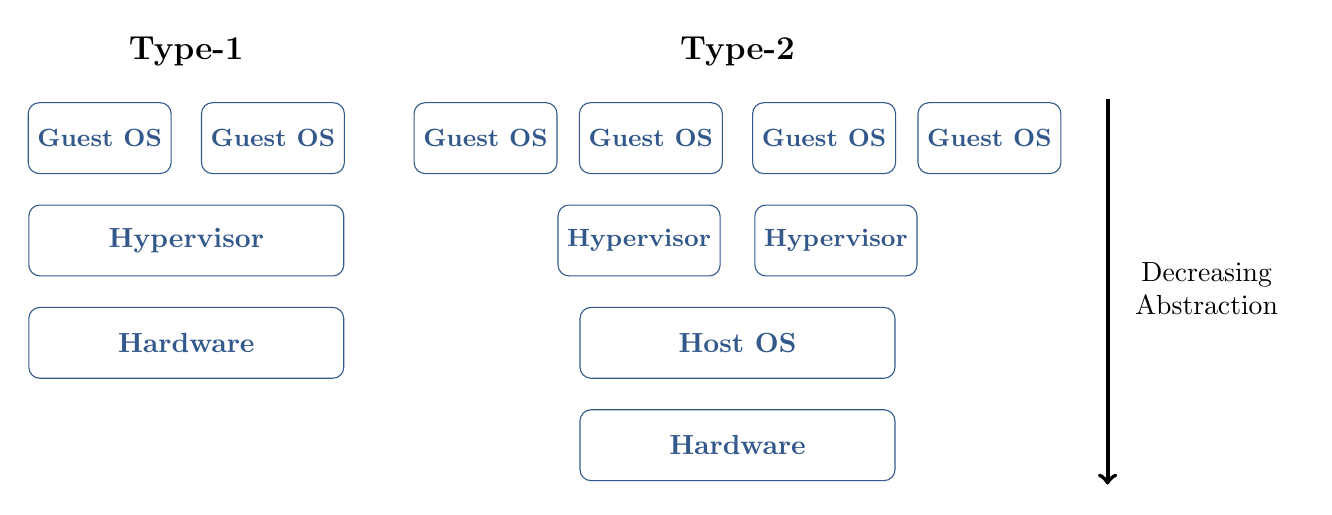
\begin{tikzpicture}[
            box/.style={
                draw=tugblue,
                rectangle,
                minimum height=0.9cm,
                align=center,
                rounded corners=4pt,
                line width=0.4pt,
                text=tugblue
            },
            hardware/.style={box, minimum width=4cm, font=\bfseries},
            hostos/.style={box, minimum width=4cm, font=\bfseries},
            hypervisor/.style={box, minimum width=4cm, font=\bfseries},
            guestos/.style={box, minimum width=1.8cm, font=\bfseries\small},
            smhypervisor/.style={box, minimum width=1.9cm, font=\bfseries\small},
            title/.style={font=\bfseries\large}
        ]

        \node[title]      at (0, 5)        {Type-1};
        \node[hardware]   at (0, 1.3)          {Hardware};
        \node[hypervisor] at (0, 2.6)        {Hypervisor};
        \node[guestos]    at (-1.1, 3.9)     {Guest OS};
        \node[guestos]    at ( 1.1, 3.9)     {Guest OS};

        \node[title]      at (7.0, 5)      {Type-2};
        \node[hardware]   at (7.0, 0)        {Hardware};
        \node[hostos]     at (7.0, 1.3)      {Host OS};
        \node[smhypervisor] at (5.75, 2.6)   {Hypervisor};
        \node[smhypervisor] at (8.25, 2.6)   {Hypervisor};
        \node[guestos]    at (3.8, 3.9)     {Guest OS};
        \node[guestos]    at (5.9, 3.9)     {Guest OS};
        \node[guestos]    at (8.1, 3.9)     {Guest OS};
        \node[guestos]    at (10.2, 3.9)    {Guest OS};

        \draw[->, line width=1.5pt] (11.7,4.4) -- (11.7,-0.5) node[midway, right] {
            \begin{tabular}{c}
            Decreasing \\
            Abstraction
            \end{tabular}
            };
        \end{tikzpicture}
        \caption{Architectural comparison of type-1 and type-2 hypervisors.}
        \label{fig:hypervisor-types}
    \end{figure}
    \noindent Modern virtualisation technologies have evolved to minimise overhead and improve
     performance for both types of hypervisors. For instance, 
     hardware-assisted virtualisation features such as 
     Intel VT-x and AMD-V have been introduced to enhance the performance
      of virtual machines by allowing certain instructions to be executed 
      directly on the physical CPU, reducing the need for VMM intervention 
      \parencite{smalleyWhatAreHypervisors2024}. Additionally, advancements 
      in memory management and I/O virtualisation have further improved the 
      efficiency of virtualised environments \parencite{barhamXenArtVirtualization2003}. However, the question of whether 
      measurable difference remain and under what workload conditions is the 
      central concern of this paper.\\
    \\
    \noindent This paper presents a comparative performance evaluation of 
    type-1 and type-2 hypervisor technologies under controlled laboratory benchmarks. 
    The methodology, results and analysis that follow aim to determine whether the 
    theoretical performance advantage of type-1 hypervisors is still observable 
    in practice today.
    \section{Methodology}

    \subsection{Test Environment}

    All benchmarks were conducted on a single physical host machine to ensure
    consistency across both hypervisor configurations. The host hardware
    specifications are detailed in Table~\ref{tab:hardware}.

    \begin{table}[H]
    \centering
    \caption{Host machine hardware specifications.}
    \label{tab:hardware}
    \begin{tabular}{ll}
    \hline
    \textbf{Component} & \textbf{Specification} \\
    \hline
    CPU    & Intel Core i5-13600K (14 cores, 20 threads) \\
    RAM    & 64 GB DDR4 @ 3200 MHz \\
    Storage & Seagate Barracuda 2TB HDD (ST2000DM008, SATA III, 7200 RPM) \\
    OS (Type 2 host) & Microsoft Windows 11 25H2 (Build 26200.8524) \\
    \hline
    \end{tabular}
    \end{table}

    \subsection{Hypervisor Configuration}

    Two hypervisors were selected to represent each architectural type:

    \begin{itemize}
        \item \textbf{Type-1: Proxmox VE 9.2-1.} Proxmox VE uses KVM as its virtualisation
         backend and is classified as a Type 1 hypervisor 
        \parencite{djordjevicPerformanceComparisonKVM2022}. It was installed directly on the
        physical hardware with no general purpose host OS present. Accessed at \url{https://enterprise.proxmox.com/iso/proxmox-ve_9.2-1.iso}.

        \item \textbf{Type-2: Oracle VirtualBox 7.2.8.} VirtualBox was installed
        on the Windows 11 host OS. As a hosted hypervisor, VirtualBox relies on
        Windows for hardware access, introducing an additional software layer
        between the guest VM and physical hardware. This is the architectural
        source of overhead being measured in this experiment. Accessed at \url{https://download.virtualbox.org/virtualbox/7.2.8/VirtualBox-7.2.8-173730-Win.exe}.
    \end{itemize}

    \subsection{Virtual Machine Configuration}

    To isolate hypervisor architecture as the sole independent variable, both
    virtual machines were configured identically across all parameters. The
    guest operating system was \textbf{Ubuntu Server 26.04 LTS} in both cases,
    installed from the same ISO image and accessed at \url{https://releases.ubuntu.com/26.04/ubuntu-26.04-live-server-amd64.iso}. The VM specifications are summarised in 
    Table~\ref{tab:vmspecs}.

    \begin{table}[H]
    \centering
    \caption{Virtual machine configuration for both hypervisors.}
    \label{tab:vmspecs}
    \begin{tabular}{ll}
    \hline
    \textbf{Parameter} & \textbf{Value} \\
    \hline
    vCPUs            & 4 \\
    RAM              & 8 GB \\
    Disk size        & 50 GB (fixed/pre-allocated) \\
    Disk controller  & SATA \\
    Firmware         & BIOS \\
    Guest OS         & Ubuntu Server 26.04 LTS \\
    \hline
    \end{tabular}
    \end{table}

    \noindent The disk was allocated as a fixed size image on both hypervisors rather than
    dynamically allocated, to eliminate allocation time overhead from
    influencing I/O benchmark results. The same disk controller type (SATA) was
    used on both VMs to avoid introducing paravirtualised driver advantages. By default,
    Proxmox VE pre-configures with VirtIO SCSI, which would give it an
    unfair I/O advantage and confound the comparison.\\
    \\
    \noindent Swap was disabled on both VMs prior to benchmarking (\texttt{sudo swapoff
    -a}) to ensure that memory benchmark results reflect RAM throughput
    exclusively, without spilling to disk.

    \subsection{Benchmark Tools}

    Two common benchmarking tools were used:

    \begin{itemize}
        \item \textbf{sysbench} — used for CPU and memory benchmarks. For the purpose of this experiment, the version used was $1.0.20$.
        \item \textbf{fio} — used for disk I/O benchmarks. For the purpose of this experiment, the version used was $3.41$.
    \end{itemize}

    \noindent Both tools were installed from the Ubuntu package repositories on each VM
    independently.

    \subsection{Benchmark Procedures}

    Each benchmark was executed five times per VM, and the arithmetic mean of
    the five runs was taken as the reported result. Prior to each test session,
    the VM was booted and left idle for two minutes to allow background OS
    processes to settle. No other VMs or applications were running on the host
    during any test.

    \subsubsection{CPU Benchmark}

    The sysbench CPU benchmark was used to measure computational throughput.
    The test calculates prime numbers up to a configurable upper bound using
    all available vCPU threads, and reports the number of events completed per
    second.

    \begin{lstlisting}[caption={sysbench CPU benchmark command.}]
    sysbench cpu --cpu-max-prime=20000 --threads=4 --time=60 run
    \end{lstlisting}

    \noindent The \texttt{--threads=4} parameter matches the vCPU allocation of each VM,
    and the test duration was fixed at 60 seconds.

    \subsubsection{Memory Benchmark}

    The sysbench memory benchmark was used to measure memory subsystem
    throughput. The test performs sequential read and write operations using
    1 MB blocks until a total transfer of 10 GB has been completed, reporting
    throughput in MiB/s.

    \begin{lstlisting}[caption={sysbench memory benchmark command.}]
    sysbench memory --memory-block-size=1M --memory-total-size=10G --threads=4 run
    \end{lstlisting}

    \subsubsection{Disk I/O Benchmark}

    Disk I/O performance was evaluated using fio with 4K random read and
    random write workloads, as small random I/O is the pattern most sensitive
    to hypervisor overhead. The I/O engine used was libaio (Linux
    asynchronous I/O), with 4 parallel jobs matching the vCPU count.\\
    \\
    \noindent A throwaway fio run was performed before each workload type to prepare
    the disk cache, ensuring that subsequent measurements reflect steady I/O
    performance rather than cold cache behaviour. The warmup run uses the same
    name as the benchmark it precedes so that fio reuses the pre-created files
    during the actual benchmark runs. After the random read warmup and five
    benchmark runs, the randread files were deleted before performing the
    random write warmup.

    \begin{lstlisting}[caption={fio random read benchmark command.}]
    fio --name=randread --ioengine=libaio --rw=randread \
        --bs=4k --size=64M --numjobs=4 --runtime=60 \
        --direct=1 --group_reporting
    \end{lstlisting}

    \begin{lstlisting}[caption={fio random write benchmark command.}]
    fio --name=randwrite --ioengine=libaio --rw=randwrite \
        --bs=4k --size=64M --numjobs=4 --runtime=60 \
        --direct=1 --group_reporting
    \end{lstlisting}

    \subsection{Controlled Variables}

    Table~\ref{tab:controls} summarises the variables held constant across both
    test environments to ensure the validity of the comparison.

    \begin{table}[H]
    \centering
    \caption{Controlled variables across both hypervisor configurations.}
    \label{tab:controls}
    \begin{tabular}{ll}
    \hline
    \textbf{Variable} & \textbf{Control measure} \\
    \hline
    Guest OS            & Identical Ubuntu Server 26.04 LTS install \\
    vCPU count          & 4 on both VMs \\
    RAM allocation      & 8 GB on both VMs \\
    Disk size           & 50 GB fixed allocation on both VMs \\
    Disk controller     & SATA on both VMs \\
    Firmware type       & BIOS on both VMs \\
    Swap               & Disabled on both VMs \\
    Concurrent load     & No other VMs or applications running \\
    Idle period         & 2 minutes post-boot before each test session \\
    Benchmark commands  & Identical commands on both VMs \\
    Run count           & 5 runs per benchmark; arithmetic mean reported \\
    \hline
    \end{tabular}
    \end{table}
    \section{Results}

    \subsection{Visualisation Methodology}

    Each benchmark subsection presents results using a radar chart, which allows
    multiple heterogeneous performance metrics to be compared simultaneously on a
    single figure. Because the metrics differ in unit and magnitude, all values are
    normalised to the dimensionless range $[0, 1]$ before plotting.\\ 
    \\
    \noindent Let $m_i$ denote the arithmetic mean of metric $i$ across the five benchmark
    runs, and let $R_i > 0$ be a predefined reference maximum for that metric.
    The normalised score $\hat{s}_i$ is given by:

    \begin{equation}
        \hat{s}_i = \frac{m_i}{R_i},\text{ where }\hat{s}_i \in [0, 1]
        \label{eq:normalise}
    \end{equation}

    \noindent The reference maximum $R_i$ for each metric is chosen as a
    conservative upper bound that strictly exceeds all observed values across both
    hypervisor configurations, i.e.:

    \begin{equation}
        R_i = \kappa \cdot \max\bigl(m_i^{\,\text{VBox}},\; m_i^{\,\text{Proxmox}}\bigr),
        \text{ where }\kappa > 1
        \label{eq:refmax}
    \end{equation}

    \noindent where $\kappa$ is a headroom factor chosen such that no data point
    saturates its axis, ensuring the full scale of the chart remains interpretable.
    The identical reference maxima are applied to both hypervisors, guaranteeing
    that the two polygons are directly comparable.\\
    \\
    \noindent For metrics where a lower value indicates better performance (e.g.\
    latency, standard deviation), the score is inverted so that a larger enclosed
    polygon area consistently represents superior performance across all axes:

    \begin{equation}
        \hat{s}_i^{\,\text{inv}} = 1 - \hat{s}_i = 1 - \frac{m_i}{R_i}
        \label{eq:invert}
    \end{equation}

    \noindent Equations~\eqref{eq:normalise}--\eqref{eq:invert} are applied
    uniformly across the CPU, memory, and disk I/O benchmark sections that follow.

    \subsection{CPU Benchmarks}

    \begin{figure}[H]
    \centering
    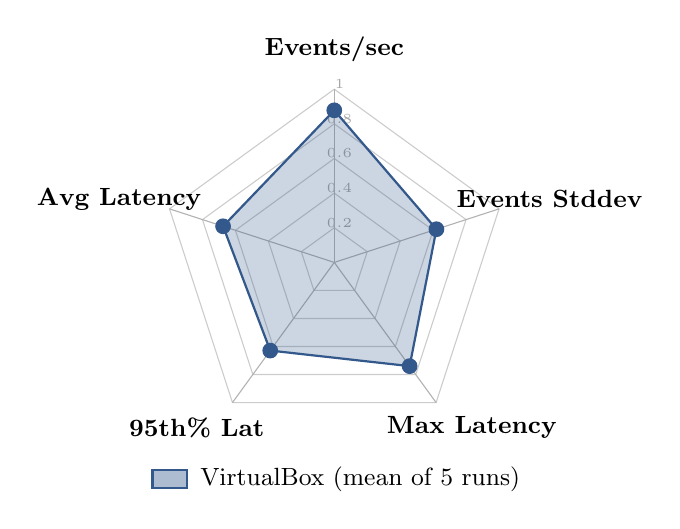
\begin{tikzpicture}[scale=2.2]
      \def\N{5}
      \def\R{1.0} 
      \def\levels{5}

      \def\LabA{Events/sec}
      \def\LabB{Avg Latency}
      \def\LabC{95th\% Lat}
      \def\LabD{Max Latency}
      \def\LabE{Events Stddev}

      \def\vboxA{0.878}
      \def\vboxB{0.675}
      \def\vboxC{0.629}
      \def\vboxD{0.740}
      \def\vboxE{0.620}

      \def\pmxA{0.0}
      \def\pmxB{0.0}
      \def\pmxC{0.0}
      \def\pmxD{0.0}
      \def\pmxE{0.0}

      \def\angleA{90}
      \def\angleB{162}
      \def\angleC{234}
      \def\angleD{306}
      \def\angleE{18}

      \foreach \lvl in {1,...,\levels}{
        \pgfmathsetmacro{\r}{\lvl/\levels*\R}
        \draw[gray!40, thin] 
          ({\r*cos(\angleA)}, {\r*sin(\angleA)}) --
          ({\r*cos(\angleB)}, {\r*sin(\angleB)}) --
          ({\r*cos(\angleC)}, {\r*sin(\angleC)}) --
          ({\r*cos(\angleD)}, {\r*sin(\angleD)}) --
          ({\r*cos(\angleE)}, {\r*sin(\angleE)}) -- cycle;
        \node[gray!70, font=\tiny] at ({0.03}, {\r+0.03}) {\pgfmathprintnumber[fixed,precision=1]{\r}};
      }

      \foreach \ang in {\angleA,\angleB,\angleC,\angleD,\angleE}{
        \draw[gray!60, thin] (0,0) -- ({\R*cos(\ang)}, {\R*sin(\ang)});
      }

      \pgfmathsetmacro{\labelR}{\R+0.18}
      \node[font=\small\bfseries, align=center] at ({\labelR*cos(\angleA)}, {\labelR*sin(\angleA)+0.05}) {\LabA};
      \node[font=\small\bfseries, align=center] at ({\labelR*cos(\angleB)-0.12}, {\labelR*sin(\angleB)}) {\LabB};
      \node[font=\small\bfseries, align=center] at ({\labelR*cos(\angleC)-0.10}, {\labelR*sin(\angleC)}) {\LabC};
      \node[font=\small\bfseries, align=center] at ({\labelR*cos(\angleD)+0.10}, {\labelR*sin(\angleD)}) {\LabD};
      \node[font=\small\bfseries, align=center] at ({\labelR*cos(\angleE)+0.12}, {\labelR*sin(\angleE)}) {\LabE};

      \draw[tugblue, thick, fill=tugblue, fill opacity=0.25]
        ({\vboxA*cos(\angleA)}, {\vboxA*sin(\angleA)}) --
        ({\vboxB*cos(\angleB)}, {\vboxB*sin(\angleB)}) --
        ({\vboxC*cos(\angleC)}, {\vboxC*sin(\angleC)}) --
        ({\vboxD*cos(\angleD)}, {\vboxD*sin(\angleD)}) --
        ({\vboxE*cos(\angleE)}, {\vboxE*sin(\angleE)}) -- cycle;

      \foreach \score/\ang in {\vboxA/\angleA, \vboxB/\angleB, \vboxC/\angleC, \vboxD/\angleD, \vboxE/\angleE}{
        \filldraw[tugblue] ({\score*cos(\ang)}, {\score*sin(\ang)}) circle (1.2pt);
      }

      \fill[tugblue, opacity=0.4] (-1.05,-1.30) rectangle (-0.85,-1.20);
      \draw[tugblue, thick]       (-1.05,-1.30) rectangle (-0.85,-1.20);
      \node[right, font=\small] at (-0.83,-1.25) {VirtualBox (mean of 5 runs)};

    \end{tikzpicture}
    \caption{VirtualBox CPU benchmark performance radar chart.}
    \label{fig:cpu-radar}
    \end{figure}

    \noindent Figure~\ref{fig:cpu-radar} shows the normalised performance profile of
    VirtualBox across five CPU metrics. Scores are computed using
    Equations~\eqref{eq:normalise}--\eqref{eq:invert}, with the following reference
    maxima: Events/sec $R = 7{,}000$; Average Latency $R = 2$\,ms; 95th Percentile
    Latency $R = 2$\,ms; Maximum Latency $R = 20$\,ms; Standard Deviation $R = 500$.
    Latency and standard deviation axes are inverted per Equation~\eqref{eq:invert},
    such that a larger enclosed area indicates better overall performance.
    \subsection{Memory Benchmarks}

    \begin{figure}[H]
    \centering
    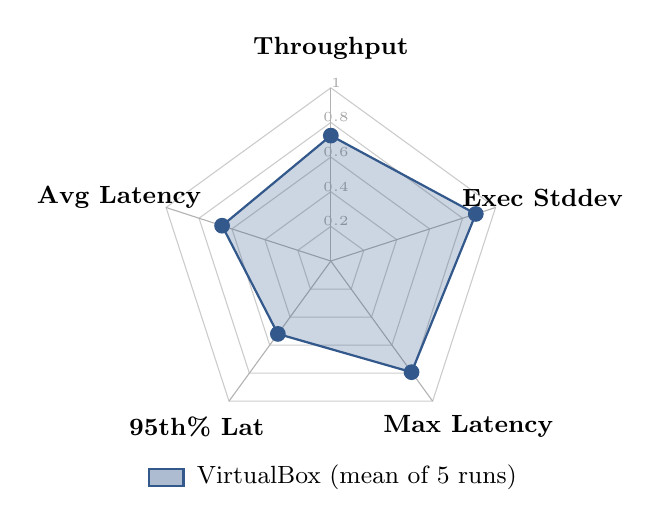
\begin{tikzpicture}[scale=2.2]

      \def\R{1.0}
      \def\levels{5}

      \def\vboxA{0.724}
      \def\vboxB{0.660}
      \def\vboxC{0.520}
      \def\vboxD{0.793}
      \def\vboxE{0.880}

      \def\pmxA{0.0}
      \def\pmxB{0.0}
      \def\pmxC{0.0}
      \def\pmxD{0.0}
      \def\pmxE{0.0}

      \def\angleA{90}
      \def\angleB{162}
      \def\angleC{234}
      \def\angleD{306}
      \def\angleE{18}

      \foreach \lvl in {1,...,\levels}{
        \pgfmathsetmacro{\r}{\lvl/\levels*\R}
        \draw[gray!40, thin]
          ({\r*cos(\angleA)}, {\r*sin(\angleA)}) --
          ({\r*cos(\angleB)}, {\r*sin(\angleB)}) --
          ({\r*cos(\angleC)}, {\r*sin(\angleC)}) --
          ({\r*cos(\angleD)}, {\r*sin(\angleD)}) --
          ({\r*cos(\angleE)}, {\r*sin(\angleE)}) -- cycle;
        \node[gray!70, font=\tiny] at ({0.03}, {\r+0.03}) {\pgfmathprintnumber[fixed,precision=1]{\r}};
      }

      \foreach \ang in {\angleA,\angleB,\angleC,\angleD,\angleE}{
        \draw[gray!60, thin] (0,0) -- ({\R*cos(\ang)}, {\R*sin(\ang)});
      }

      \pgfmathsetmacro{\labelR}{\R+0.18}
      \node[font=\small\bfseries, align=center] at ({\labelR*cos(\angleA)},   {\labelR*sin(\angleA)+0.05})  {Throughput};
      \node[font=\small\bfseries, align=center] at ({\labelR*cos(\angleB)-0.10}, {\labelR*sin(\angleB)})   {Avg Latency};
      \node[font=\small\bfseries, align=center] at ({\labelR*cos(\angleC)-0.08}, {\labelR*sin(\angleC)})   {95th\% Lat};
      \node[font=\small\bfseries, align=center] at ({\labelR*cos(\angleD)+0.10}, {\labelR*sin(\angleD)})   {Max Latency};
      \node[font=\small\bfseries, align=center] at ({\labelR*cos(\angleE)+0.10}, {\labelR*sin(\angleE)})   {Exec Stddev};

      \draw[tugblue, thick, fill=tugblue, fill opacity=0.25]
        ({\vboxA*cos(\angleA)}, {\vboxA*sin(\angleA)}) --
        ({\vboxB*cos(\angleB)}, {\vboxB*sin(\angleB)}) --
        ({\vboxC*cos(\angleC)}, {\vboxC*sin(\angleC)}) --
        ({\vboxD*cos(\angleD)}, {\vboxD*sin(\angleD)}) --
        ({\vboxE*cos(\angleE)}, {\vboxE*sin(\angleE)}) -- cycle;

      \foreach \score/\ang in {\vboxA/\angleA,\vboxB/\angleB,\vboxC/\angleC,\vboxD/\angleD,\vboxE/\angleE}{
        \filldraw[tugblue] ({\score*cos(\ang)}, {\score*sin(\ang)}) circle (1.2pt);
      }

      \fill[tugblue, opacity=0.4] (-1.05,-1.30) rectangle (-0.85,-1.20);
      \draw[tugblue, thick]       (-1.05,-1.30) rectangle (-0.85,-1.20);
      \node[right, font=\small] at (-0.83,-1.25) {VirtualBox (mean of 5 runs)};

    \end{tikzpicture}
    \caption{VirtualBox memory benchmark performance radar chart.}
    \label{fig:mem-radar}
    \end{figure}

    \noindent Figure~\ref{fig:mem-radar} shows the normalised memory performance
    profile of VirtualBox across five metrics. Scores are computed using
    Equations~\eqref{eq:normalise}--\eqref{eq:invert}, with the following reference
    maxima: Throughput $R = 120{,}000$\,MiB/s; Average Latency $R = 0.10$\,ms;
    95th Percentile Latency $R = 0.10$\,ms; Maximum Latency $R = 15$\,ms;
    Execution Standard Deviation $R = 0.05$. Latency and standard deviation axes
    are inverted per Equation~\eqref{eq:invert}.

    \subsection{Disk I/O Benchmarks}

    \begin{figure}[H]
    \centering
    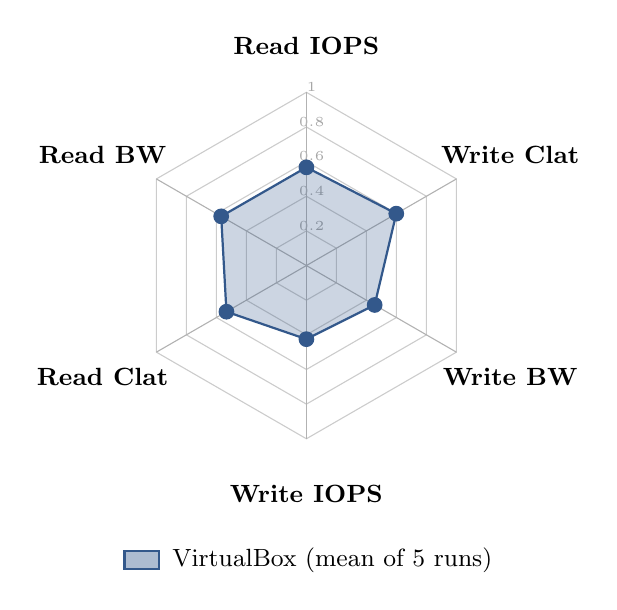
\begin{tikzpicture}[scale=2.2]

      \def\R{1.0}
      \def\levels{5}

      \def\vboxA{0.567}
      \def\vboxB{0.568}
      \def\vboxC{0.533}
      \def\vboxD{0.425}
      \def\vboxE{0.455}
      \def\vboxF{0.599}

      \def\pmxA{0.0}
      \def\pmxB{0.0}
      \def\pmxC{0.0}
      \def\pmxD{0.0}
      \def\pmxE{0.0}
      \def\pmxF{0.0}

      \def\angleA{90}
      \def\angleB{150}
      \def\angleC{210}
      \def\angleD{270}
      \def\angleE{330}
      \def\angleF{30}

      \foreach \lvl in {1,...,\levels}{
        \pgfmathsetmacro{\r}{\lvl/\levels*\R}
        \draw[gray!40, thin]
          ({\r*cos(\angleA)}, {\r*sin(\angleA)}) --
          ({\r*cos(\angleB)}, {\r*sin(\angleB)}) --
          ({\r*cos(\angleC)}, {\r*sin(\angleC)}) --
          ({\r*cos(\angleD)}, {\r*sin(\angleD)}) --
          ({\r*cos(\angleE)}, {\r*sin(\angleE)}) --
          ({\r*cos(\angleF)}, {\r*sin(\angleF)}) -- cycle;
        \node[gray!70, font=\tiny] at ({0.03}, {\r+0.03}) {\pgfmathprintnumber[fixed,precision=1]{\r}};
      }

      \foreach \ang in {\angleA,\angleB,\angleC,\angleD,\angleE,\angleF}{
        \draw[gray!60, thin] (0,0) -- ({\R*cos(\ang)}, {\R*sin(\ang)});
      }

      \pgfmathsetmacro{\labelR}{\R+0.22}
      \node[font=\small\bfseries, align=center] at ({\labelR*cos(\angleA)},        {\labelR*sin(\angleA)+0.05})  {Read IOPS};
      \node[font=\small\bfseries, align=center] at ({\labelR*cos(\angleB)-0.12},   {\labelR*sin(\angleB)+0.03})  {Read BW};
      \node[font=\small\bfseries, align=center] at ({\labelR*cos(\angleC)-0.12},   {\labelR*sin(\angleC)-0.03})  {Read Clat};
      \node[font=\small\bfseries, align=center] at ({\labelR*cos(\angleD)},        {\labelR*sin(\angleD)-0.10})  {Write IOPS};
      \node[font=\small\bfseries, align=center] at ({\labelR*cos(\angleE)+0.12},   {\labelR*sin(\angleE)-0.03})  {Write BW};
      \node[font=\small\bfseries, align=center] at ({\labelR*cos(\angleF)+0.12},   {\labelR*sin(\angleF)+0.03})  {Write Clat};

      \draw[tugblue, thick, fill=tugblue, fill opacity=0.25]
        ({\vboxA*cos(\angleA)}, {\vboxA*sin(\angleA)}) --
        ({\vboxB*cos(\angleB)}, {\vboxB*sin(\angleB)}) --
        ({\vboxC*cos(\angleC)}, {\vboxC*sin(\angleC)}) --
        ({\vboxD*cos(\angleD)}, {\vboxD*sin(\angleD)}) --
        ({\vboxE*cos(\angleE)}, {\vboxE*sin(\angleE)}) --
        ({\vboxF*cos(\angleF)}, {\vboxF*sin(\angleF)}) -- cycle;

      \foreach \score/\ang in {\vboxA/\angleA,\vboxB/\angleB,\vboxC/\angleC,\vboxD/\angleD,\vboxE/\angleE,\vboxF/\angleF}{
        \filldraw[tugblue] ({\score*cos(\ang)}, {\score*sin(\ang)}) circle (1.2pt);
      }

      \fill[tugblue, opacity=0.4] (-1.05,-1.75) rectangle (-0.85,-1.65);
      \draw[tugblue, thick]       (-1.05,-1.75) rectangle (-0.85,-1.65);
      \node[right, font=\small] at (-0.83,-1.70) {VirtualBox (mean of 5 runs)};

    \end{tikzpicture}
    \caption{VirtualBox disk I/O benchmark performance radar chart.}
    \label{fig:io-radar}
    \end{figure}

    \noindent Figure~\ref{fig:io-radar} shows the normalised disk I/O performance
    profile of VirtualBox across six metrics covering both random read and random
    write workloads. Scores are computed using
    Equations~\eqref{eq:normalise}--\eqref{eq:invert}, with the following reference
    maxima: Read IOPS $R = 500$; Read Bandwidth $R = 2{,}000$\,KiB/s; Read
    Completion Latency $R = 30{,}000\,\mu$s; Write IOPS $R = 400$; Write Bandwidth
    $R = 1{,}500$\,KiB/s; Write Completion Latency $R = 60{,}000\,\mu$s.
    Completion latency axes are inverted per Equation~\eqref{eq:invert}.
    \section{Discussion}
    \section{Conclusion}
    \newpage
    \printbibliography
    \newpage
    \begin{landscape}
    \appendix
    \section*{Appendices}
    \addcontentsline{toc}{section}{Appendices}
    \section{CPU Benchmark Results}
    \begin{table}[H]
    \centering
    \caption{VirtualBox CPU benchmark results (sysbench, 5 runs).}
    \label{tab:cpu-vbox}
    \begin{tabular}{lrrrrrrr}
    \hline
    \textbf{Run} & \textbf{Events/sec} & \textbf{Total Events} & \textbf{Min Lat (ms)} & \textbf{Avg Lat (ms)} & \textbf{Max Lat (ms)} & \textbf{95th\% (ms)} & \textbf{Events Stddev} \\
    \hline
    1 & 6138.21 & 368301 & 0.62 & 0.65 & 7.31  & 0.74 & 101.23 \\
    2 & 6177.91 & 370689 & 0.62 & 0.65 & 2.48  & 0.73 & 159.81 \\
    3 & 6135.72 & 368153 & 0.62 & 0.65 & 11.05 & 0.75 & 375.66 \\
    4 & 6161.86 & 369721 & 0.62 & 0.65 & 2.46  & 0.74 & 124.00 \\
    5 & 6102.55 & 366163 & 0.62 & 0.65 & 2.69  & 0.75 & 189.52 \\
    \hline
    \textbf{Mean} & \textbf{6143.25} & \textbf{368605} & \textbf{0.62} & \textbf{0.65} & \textbf{5.20} & \textbf{0.742} & \textbf{190.04} \\
    \hline
    \end{tabular}
    \end{table}

    \begin{table}[H]
    \centering
    \caption{Proxmox CPU benchmark results (sysbench, 5 runs).}
    \label{tab:cpu-proxmox}
    \begin{tabular}{lrrrrrrr}
    \hline
    \textbf{Run} & \textbf{Events/sec} & \textbf{Total Events} & \textbf{Min Lat (ms)} & \textbf{Avg Lat (ms)} & \textbf{Max Lat (ms)} & \textbf{95th\% (ms)} & \textbf{Events Stddev} \\
    \hline
    1 & & & & & & & \\
    2 & & & & & & & \\
    3 & & & & & & & \\
    4 & & & & & & & \\
    5 & & & & & & & \\
    \hline
    \textbf{Mean} & & & & & & & \\
    \hline
    \end{tabular}
    \end{table}
    \end{landscape}

    \begin{landscape}
    \section{Memory Benchmark Results}
    \begin{table}[H]
    \centering
    \caption{VirtualBox memory benchmark results (sysbench, 5 runs).}
    \label{tab:mem-vbox}
    \begin{tabular}{lrrrrrrr}
    \hline
    \textbf{Run} & \textbf{Throughput (MiB/s)} & \textbf{Total Ops} & \textbf{Min Lat (ms)} & \textbf{Avg Lat (ms)} & \textbf{Max Lat (ms)} & \textbf{95th\% (ms)} & \textbf{Exec Stddev} \\
    \hline
    1 & 106235.51 & 10240 & 0.02 & 0.03 & 3.17  & 0.04 & 0.00 \\
    2 &  67435.16 & 10240 & 0.02 & 0.03 & 0.22  & 0.05 & 0.01 \\
    3 &  69355.60 & 10240 & 0.02 & 0.03 & 0.19  & 0.04 & 0.01 \\
    4 & 103618.39 & 10240 & 0.02 & 0.04 & 1.47  & 0.07 & 0.00 \\
    5 &  87759.48 & 10240 & 0.02 & 0.04 & 10.45 & 0.04 & 0.01 \\
    \hline
    \textbf{Mean} & \textbf{86880.83} & \textbf{10240} & \textbf{0.02} & \textbf{0.034} & \textbf{3.10} & \textbf{0.048} & \textbf{0.006} \\
    \hline
    \end{tabular}
    \end{table}

    \begin{table}[H]
    \centering
    \caption{Proxmox memory benchmark results (sysbench, 5 runs).}
    \label{tab:mem-proxmox}
    \begin{tabular}{lrrrrrrr}
    \hline
    \textbf{Run} & \textbf{Throughput (MiB/s)} & \textbf{Total Ops} & \textbf{Min Lat (ms)} & \textbf{Avg Lat (ms)} & \textbf{Max Lat (ms)} & \textbf{95th\% (ms)} & \textbf{Exec Stddev} \\
    \hline
    1 & & & & & & & \\
    2 & & & & & & & \\
    3 & & & & & & & \\
    4 & & & & & & & \\
    5 & & & & & & & \\
    \hline
    \textbf{Mean} & & & & & & & \\
    \hline
    \end{tabular}
    \end{table}
    \end{landscape}

    \begin{landscape}
    \section{Disk I/O Benchmark Results}
    \begin{table}[H]
    \centering
    \caption{VirtualBox random read disk I/O benchmark results (fio, 5 runs).}
    \label{tab:io-read-vbox}
    \begin{tabular}{lrrrrrrrrr}
    \hline
    \textbf{Run} & \textbf{IOPS} & \textbf{BW (KiB/s)} & \textbf{Avg BW (KiB/s)} & \textbf{Avg IOPS} & \textbf{BW Stdev (KiB/s)} & \textbf{IOPS Stdev} & \textbf{Avg Clat ($\mu$s)} & \textbf{Clat Stdev ($\mu$s)} \\
    \hline
    1 & 291 & 1167 & 1165.61 & 290.20 & 51.85 & 12.97 & 13608.85 & 14213.95 \\
    2 & 278 & 1113 & 1114.32 & 277.19 & 52.09 & 13.01 & 14274.81 & 15848.32 \\
    3 & 269 & 1076 & 1075.96 & 267.15 & 52.86 & 13.24 & 14771.76 & 16303.08 \\
    4 & 282 & 1130 & 1129.46 & 280.81 & 48.03 & 12.04 & 14048.93 & 14851.57 \\
    5 & 297 & 1190 & 1191.12 & 296.57 & 55.46 & 13.87 & 13337.12 & 15130.93 \\
    \hline
    \textbf{Mean} & \textbf{283.4} & \textbf{1135.2} & \textbf{1135.29} & \textbf{282.38} & \textbf{52.06} & \textbf{13.03} & \textbf{14008.29} & \textbf{15269.57} \\
    \hline
    \end{tabular}
    \end{table}

    \begin{table}[H]
    \centering
    \caption{Proxmox random read disk I/O benchmark results (fio, 5 runs).}
    \label{tab:io-read-proxmox}
    \begin{tabular}{lrrrrrrrrr}
    \hline
    \textbf{Run} & \textbf{IOPS} & \textbf{BW (KiB/s)} & \textbf{Avg BW (KiB/s)} & \textbf{Avg IOPS} & \textbf{BW Stdev (KiB/s)} & \textbf{IOPS Stdev} & \textbf{Avg Clat ($\mu$s)} & \textbf{Clat Stdev ($\mu$s)} \\
    \hline
    1 & & & & & & & & \\
    2 & & & & & & & & \\
    3 & & & & & & & & \\
    4 & & & & & & & & \\
    5 & & & & & & & & \\
    \hline
    \textbf{Mean} & & & & & & & & \\
    \hline
    \end{tabular}
    \end{table}

    \begin{table}[H]
    \centering
    \caption{VirtualBox random write disk I/O benchmark results (fio, 5 runs).}
    \label{tab:io-write-vbox}
    \begin{tabular}{lrrrrrrrrr}
    \hline
    \textbf{Run} & \textbf{IOPS} & \textbf{BW (KiB/s)} & \textbf{Avg BW (KiB/s)} & \textbf{Avg IOPS} & \textbf{BW Stdev (KiB/s)} & \textbf{IOPS Stdev} & \textbf{Avg Clat ($\mu$s)} & \textbf{Clat Stdev ($\mu$s)} \\
    \hline
    1 & 133 & 534 & 3930.80 & 980.98  & 996.44  & 249.30 & 29862.54 & 402831.82 \\
    2 & 142 & 568 & 3032.12 & 756.62  & 917.81  & 229.52 & 28033.35 & 445593.33 \\
    3 & 178 & 713 & 5303.47 & 1324.18 & 1150.74 & 287.79 & 22326.45 & 383498.96 \\
    4 & 189 & 758 & 6071.94 & 1517.17 & 1305.09 & 326.34 & 20985.67 & 353770.39 \\
    5 & 209 & 836 & 5295.56 & 1322.22 & 1262.74 & 315.85 & 19019.98 & 316261.22 \\
    \hline
    \textbf{Mean} & \textbf{170.2} & \textbf{681.8} & \textbf{4726.78} & \textbf{1180.23} & \textbf{1126.56} & \textbf{281.76} & \textbf{24045.60} & \textbf{380391.14} \\
    \hline
    \end{tabular}
    \end{table}

    \begin{table}[H]
    \centering
    \caption{Proxmox random write disk I/O benchmark results (fio, 5 runs).}
    \label{tab:io-write-proxmox}
    \begin{tabular}{lrrrrrrrrr}
    \hline
    \textbf{Run} & \textbf{IOPS} & \textbf{BW (KiB/s)} & \textbf{Avg BW (KiB/s)} & \textbf{Avg IOPS} & \textbf{BW Stdev (KiB/s)} & \textbf{IOPS Stdev} & \textbf{Avg Clat ($\mu$s)} & \textbf{Clat Stdev ($\mu$s)} \\
    \hline
    1 & & & & & & & & \\
    2 & & & & & & & & \\
    3 & & & & & & & & \\
    4 & & & & & & & & \\
    5 & & & & & & & & \\
    \hline
    \textbf{Mean} & & & & & & & & \\
    \hline
    \end{tabular}
    \end{table}
    \end{landscape}
\end{document}